\part{Modelo Escala}

\section{Resultados}

\subsection{Calculo Permeabilidad Muestra}

\subsection{Aplicacion Diferencias Finitas}

Se determina un caudal de 0.008972885614821659 m/s

\subsection{Licuefaccion}

A continuacion se presenta un video (ver en Adobe Acrobat) de la falla observada por licuefaccion en la maqueta a escala.

\begin{center}
    \includemedia[
        width=0.5625\textwidth, % Relación de aspecto 9:16 (altura mayor que el ancho)
        height=\textwidth,
        activate=onclick,
        addresource=VIDEOS/licuefaccion.mp4,
        flashvars={
            source=VIDEOS/licuefaccion.mp4
        }
    ]{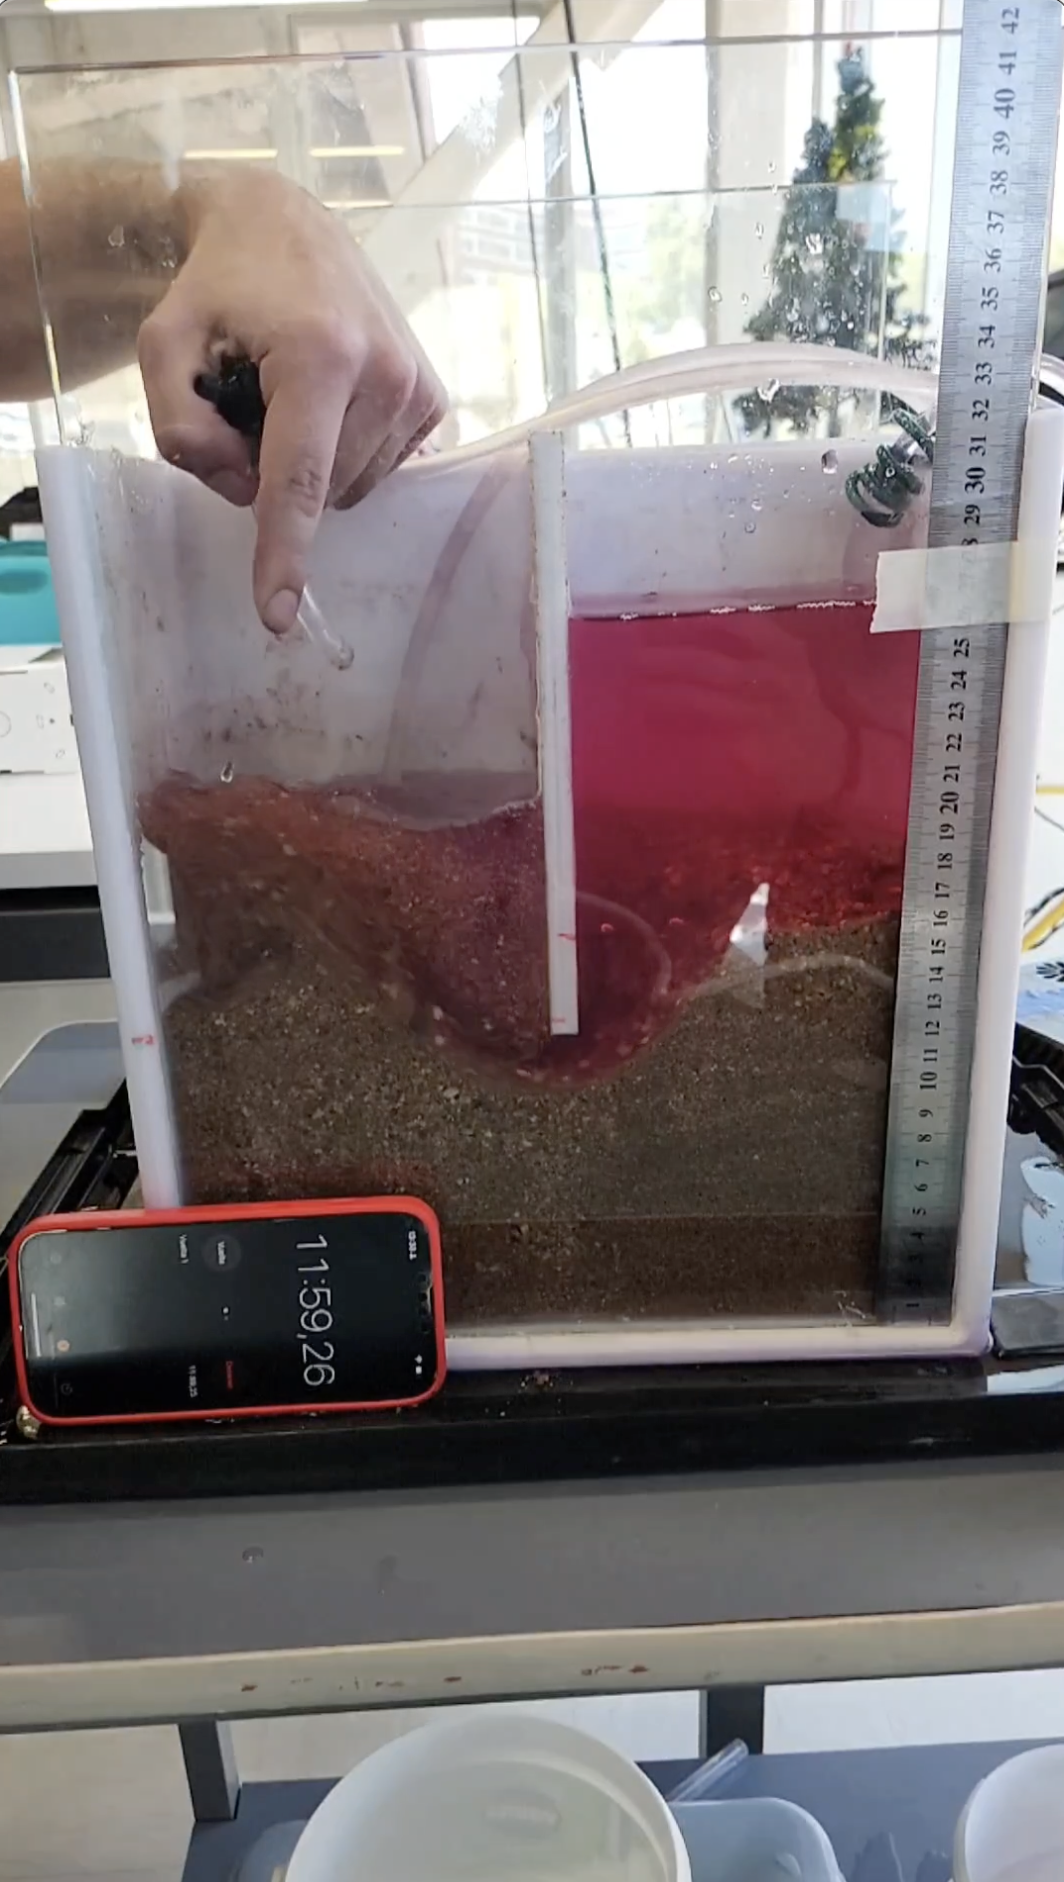
\includegraphics[width=\textwidth]{VIDEOS/miniatura_licuefaccion.png}}{VPlayer.swf}
\end{center}